% Preamble
\documentclass[a4paper,14pt]{extarticle}

% Packages
\usepackage{geometry}
\usepackage[T2A]{fontenc}
\usepackage[utf8]{inputenc}
\usepackage[english,russian]{babel}
\usepackage{amsmath}
\usepackage{amsthm}
\usepackage{amssymb}
\usepackage{fancyhdr}
\usepackage{setspace}
\usepackage{graphicx}
\usepackage{colortbl}
\usepackage{tikz}
\usepackage{pgf}
\usepackage{subcaption}
\usepackage{listings}
\usepackage[colorlinks, linkcolor=blue, urlcolor=blue]{hyperref}
\usepackage{indentfirst}

\hypersetup{
    colorlinks=true,
    linkcolor=black,
    urlcolor=blue,
}
\urlstyle{same}
\usepackage{appendix}
%\usepackage{algorithm}
\usepackage{amsfonts}
%\usepackage{algorithmicx}
%\usepackage{algpseudocode}
\usepackage{csquotes}
\usepackage{multirow}
\usepackage{booktabs}
\usepackage{longtable}
%\usepackage[sorting=nyvt, backend=bibtex, firstinits=true]{biblatex}
\usepackage[sorting=nyvt, backend=bibtex, giveninits]{biblatex}
\addbibresource{bibliography.bib}

\DeclareNameAlias{sortname}{family-given}
\DeclareNameAlias{default}{family-given}

\geometry{left=2.5cm}  % левое поле
\geometry{right=1.5cm}  % правое поле
\geometry{top=1.5cm}  % верхнее поле
\geometry{bottom=1.5cm}  % нижнее поле
\renewcommand{\baselinestretch}{1.5}  % междустрочный интервал

\renewcommand{\theenumi}{\arabic{enumi}}  % Меняем везде перечисления на цифра.цифра
\renewcommand{\labelenumi}{\arabic{enumi}}  % Меняем везде перечисления на цифра.цифра
\renewcommand{\theenumii}{.\arabic{enumii}}  % Меняем везде перечисления на цифра.цифра
\renewcommand{\labelenumii}{\arabic{enumi}.\arabic{enumii}.}  % Меняем везде перечисления на цифра.цифра
\renewcommand{\theenumiii}{.\arabic{enumiii}}  % Меняем везде перечисления на цифра.цифра
\renewcommand{\labelenumiii}{\arabic{enumi}.\arabic{enumii}.\arabic{enumiii}.}  % Меняем везде перечисления на цифра.цифра

\DeclareMathOperator*{\argmax}{arg\,max}
\newcommand{\ind}{\hspace{\algorithmicindent}}

\DeclareMathAlphabet{\pazocal}{OMS}{zplm}{m}{n}
\newcommand{\unif}{\pazocal{U}}
\graphicspath{{images/}}

\usepackage{chngcntr}
\counterwithin{figure}{section}
\counterwithin{table}{section}
%\counterwithin{algorithm}{section}
\counterwithin{equation}{section}

\makeatletter
\renewcommand*{\@Alph}[1]{\ifcase #1\or А\or Б\or В\or Г\or Д\or Е\or Ж\or З\or И\or К\or Л\or М\or Н\or О\or П\or Р\or С\or Т\or У\or Ф\or Х\or Ц\or Ч\or Ш\or Щ\or Э\or Ю\or Я\else\@ctrerr  \fi}
\makeatother

%\usepackage{lineno} % номера строк для rewiew
%\linenumbers

\DeclareMathOperator*{\Count}{Count}

% Document
\begin{document}
    \begin{titlepage}
\newpage

{\setstretch{1.0}
\begin{center}
Федеральное государственное автономное образовательное учреждение высшего образования «Национальный исследовательский университет «Высшая школа экономики»
\\
\bigskip
Факультет компьютерных наук \\
Основная образовательная программа \\
Прикладная математика и информатика \\
\end{center}
}

\vspace{8em}

\begin{center}
{\Large КУРСОВАЯ РАБОТА}\\
\textsc{\textbf{
Исследовательский проект на тему
\linebreak
"Предсказание критических событий в моделях Абелевой кучи БТВ и Манна"}}
\end{center}

\vspace{2em}

{\setstretch{1.0}
\hfill\parbox{16cm}{
\hspace*{5cm}\hspace*{-5cm}Выполнил студент группы 192, 3 курса,\\
 Сапожников Денис Сергеевич\\
 
\hspace*{5cm}\hspace*{-5cm}Руководитель КР:\\
научный сотрудник Попов Виктор Юрьевич\\

%\hspace*{5cm}\hspace*{-5cm}Куратор:\hfill < степень>, <звание>, <ФИО полностью>\\

\hspace*{5cm}\hspace*{-5cm}Соруководитель КР:\\
научный сотрудник Шаповал Александр Борисович\\
}
}

\vspace{\fill}

\begin{center}
Москва 2022
\end{center}

\end{titlepage}

    \newpage

    {
        \hypersetup{linkcolor=black}
        \tableofcontents
    }

    \newpage
    \begin{abstract}
     В моделях самоорганизованной критичности, основанных на модели <<куча песка>>, событиям, которые расположены на <<хвосте>> вероятностного распределения событий по размерам, предшествует определённое затишье. Это свойство позволяет прогнозировать время наступления таких событий, при чём прогноз становится эффективнее с увеличением размера прогнозируемых событий. В этой работе мы оценили прогнозируемость в моделях Манна и Бака-Танга-Визенфельда (БТВ) на квадратной решётке в термодинамическом пределе, когда объём системы стремится к бесконечности. Для обеих моделей реализован алгоритм, прогнозирующий наступление крупных событий после уменьшения активности. Установлено совпадение эффективности прогноза на различных решётках для каждой из моделей после нормировки размера событий степенной функцией длины решётки. Показатели степени равны $2.75$ и $3$ для моделей Манна и БТВ соответственно. Из этого следует, что в модели БТВ, в отличие от модели Манна, прогноз в термодинамическом пределе невозможен, по крайней мере на основе предшествующего затишься.
    \newline
    \newline
    Ссылка на гитхаб с проектом - \url{https://github.com/i1oveMyse1f/abel-heap}.
    \newline
    \newline
    \textbf{\textit{Ключевые слова---}} Самоорганизованные критические системы, Модель Манна, Модель БТВ, Скейлинг.
    \newpage
    The state-of-the-art in the theory of self-organized criticality exposes that a certain quiescence precedes events that are located on the tail of the probability distribution of events with respect to their sizes. The existence of the quiescence allows us to predict the occurrence of these events in advance. In this work, we estimate the predictability of the Bak-Tang-Wiesenfeld (BTW) and Manna models on the square lattice in the thermodynamic limit defined by the tendency of the system volume to infinity. For both models, we define an algorithm that forecasts the occurrence of large events after a fall in activity. The collapse of the algorithm efficiency computed with various lattices is found if the size of events is normalized by a power-law function of the lattice length. The power-law exponents are $2.75$ and $3$ for the Manna and BTW models respectively. This yields that the prediction in thermodynamic limit does not exist in the BTW but not in the Manna model, at least based on the quiescence.
    \newline
    \newline
    Github project link - \url{https://github.com/i1oveMyse1f/abel-heap}.
    \newline
    \newline
    \textbf{\textit{Keywords---}} Self-organized criticality, Manna model, BTW model, Scaliability.
\end{abstract}

    \newpage

    \section{Введение}
    В XX веке исследователи часто наблюдали степенной закон в разных физических явлениях, например, в сейсмичности~\cite{Burridge1967ModelAT}, солнечной активности~\cite{Dennis1985SolarHX}, распределении богатства~\cite{Levy1997NEWEF}. Однако, долгое время не существовало теории и математической модели для объяснения степенного закона, пока в 1987 году Бак, Танг и Винфельд не предложили теорию самоорганизованной критичности и модель песчаной кучи~\cite{btw} (\textit{англ., sandpile}), как её архитипичный пример. Модификации модели песчаной кучи применимы к моделированию сейсмичности~\cite{Khodaverdian2016,TURCOTTE1999275}, взаимодействию нейронов в мозге~\cite{Bak1996HowNW}, солнечной активности~\cite{Aschwanden2021SelforganizedCI}, естественных языков~\cite{Gromov2020} и других явлений~\cite{bunde,Kalinin2021,podgornik}.

Эволюция в модели песчаной кучи Бака–Танга–Визенфельда (БТВ)~\cite{btw} определяется на квадратной решётке со стороной в $L$ клеток. В каждой клетке находится от $0$ до $3$ песчинок. Каждый момент времени выбирается случайная клетка, в которую добавляется одна песчинка. Если в клетке оказывается $4$ песчинки или больше, то клетка называется нестабильной и происходит обвал: из нестабильной клетки в каждую из соседних клеток перемещается по одной песчинке; если соседней клетки нет, то песчинка падает за пределы решетки. Обвалы происходят, пока существуют нестабильные клетки. Считается, что обвалы происходят моментально, то есть до добавления новой песчинки на решётку. Последовательный процесс обвалов называется событием; размером $i$-го события считается количество обвалов $s_i$, которое произошло до стабилизации кучи после падения $i$-й песчинки.

Манна~\cite{manna} предложил другую реализацию модели песчаной кучи, определив стохастический процесс пересыпания песчинок вместо детерминистического. Измененные правила обвала выглядят следующим образом: из нестабильной клетки $4$ раза равновероятно выбирается случайная соседняя клетка, в которую перемещается одна песчинка. Эта модель так же позволяет наблюдать степенной закон, но c другими параметрами. Позже выяснилось, что пока геометрия решетки квадратная, а правила обвала --- симметричные, других степенных законов, отличных от моделей БТВ и Манна, получить не удаётся~\cite{BenHur1996,Dhar2006}.

За счёт простоты модели песчаной кучи удалось исследовать большое количество её свойств, которые позже наблюдались и в жизни~\cite{Held1990,Jaeger1989}. Однако часто эти свойства можно наблюдать только на больших решетках~\cite{Liu1991}. Поэтому исследователи уделяют отдельное внимание термодинамическому пределу --- свойству модели при размере решетки, стремящемуся к бесконечности. Например, выяснилось, что термодинамический предел для шкалируемости, или скейлинга, плотности событий в модели Манна равен $L^{2.75}$~\cite{manna,Vespignani2000AbsorbingstatePT,Dhar2006}. Это значит, что начиная с какого-то $L$ плотности распределений событий будут совпадать, если сжать их по оси размера событий в $L^{2.75}$ раз. Схожий результат о плотности распределения известен и в модели БТВ: размер максимального события $s_{\max} \propto L^3$~\cite{Garber2009}.

Отдельным важным вопросом в модели песчаной кучи является возможность прогнозировать критические, или крупные, события. Долгие годы считалось, что предсказывать крупные события в данной модели невозможно~\cite{Geller1997,Wyss1997,Milovanov2021}, но в последнее время появилось множество разных подходов. Например, в работе~\cite{deluca} был представлен способ прогнозирования на основе расстояния между событиями одного и того же размера для модели Манна. А в работах ~\cite{Hallerberg2009,Kantz2010} предложили использовать условную вероятность крупного события в зависимости от переменной принятия решений, содержащую информацию о предыдущих событиях для модели БТВ.

Целью нашего исследования является проведение сравнительного анализа прогнозируемости (как свойства системы) в моделях БТВ и Манна. Мы намерены описать скейлинг эффективности прогноза относительно длины решётки и оценить прогнозируемость в термодинамическом пределе для каждой из моделей.

    \newpage

    \section{Методы}
    \subsection{Данные}
Для каждой решетки размера $L \in [64, 128, 256, 512]$ мы сгенерировали выборку $\{s_i\}_{i=1}^{N}$в модели Манна и БТВ размера $N=10^8$, пропустив первые $10 \cdot L^2$ событий, чтобы насытить решетку песчинками. Затем мы разбили данные пополам на тренировочную и тестовую части.

\subsection{Модель}
Чтобы качество прогноза не зависело от стороны решетки, мы вводим шкалирование размеров прогнозируемых крупных событий $X_i = I[s_i > \eta(L)]$. Для скейлинг-фукнции $\eta(L)$ мы предлагаем формулу

$$ \eta(L) = p \cdot L^\gamma, $$

\noindent где $\gamma$ -- подбираемый параметр, который различается для моделей Манна и БТВ, а $p$ --- некоторая константа, большая $0$, не зависящая от стороны решетки и регулирующая частоту прогнозирующих событий.

\subsection{Алгоритм}

Наши прогнозы будут основаны на переменной принятия решения $y_i$, введенной в~\cite{Hallerberg2009,Kantz2010}, формула которой похожа на измененный AR(1)-процесс, изучавшийся в~\cite{Lewis1985}:

$$y_i = \sum\limits_{k=1}^{i} a^k \cdot s_{i-k}, $$

\noindent где $a$ --- подбираемый параметр, переведенный в логарифмическую шкалу: $a = \exp\left(-\frac{1}{T}\right)$~\cite{Hallerberg2009}.

На тренировочной выборке для каждой решетки по-отдельности мы оцениваем условную вероятность $P(X=1\ |\ y)$. Для этого мы разбиваем значения $y$ на $200$ равных бинов, и в каждом вычисляем условную вероятность по формуле:

$$ \hat{P}(X_i = 1\ | y_i \in y_{bin}) = \frac{\Count\limits_{j}(X_j = 1\ |\ y_{j} \in y_{bin})}{\Count\limits_{j}(X_j\ |\ y_{j} \in y_{bin})} $$

Для прогноза на тестовой выборке мы так же вычисляем перемененную принятия решения, по которой выдаем вероятность крупного события, оцененную по формуле.

\subsection{Метрики}

Для анализа качества модели мы будем использовать ROC-кривые~\cite{Molchan1997}, поскольку перед нами стоит задача бинарной классификации с несбалансированной выборкой (см. Приложение \ref{appendix:c}).  Количественной интерпретацией ROC-кривой, которую мы будем использовать для оценки алгоритма, является метрика $\epsilon(L,\gamma,p,T)$, равная Манхетонскому расстоянию от точки $(0, 1)$ до ближайшей к ней точке на ROC-кривой~\cite{Hallerberg2009,Shapoval2006}, построенной по прогнозу модели с фиксированными параметрами $L$, $\gamma$, $p$ и $T$.

Поскольку в нашей работе мы ищем шкалиремую предсказательную модель, необходимо численно оценивать качество шкалирования для разных $\gamma$. С точки зрения метрики $\epsilon$, идеальный параметр шкалирования $\gamma$ --- это тот, в результате которого для всех фиксированных $p$ качество модели $\epsilon_{\gamma,p,T}(L)$ с оптимально подобранным $T$ не зависит от $L$. Это значит, что абсолютное значение углового коэффициента $k(p, \gamma)$ регрессирующей прямой, проходящей через точки на кривой $\epsilon_{\gamma,p,T}(L)$ должен быть близок к $0$, а сами точки иметь близкую к нулю дисперсию $v(p, \gamma)$.

С другой стороны, $\epsilon$ --- это лишь одна точка на ROC-кривой, которая не позволяет сказать о качестве шкалируемости целиком. По этой причине, чтобы показать, что алгоритм обладает свойством шкалируемости, в работах~\cite{Hallerberg2009,deluca} добиваются наложения ROC-кривых. Поэтому мы предлагаем численно оценивать качество наложения ROC-кривых с помощью Intersection over Union (IoU) метрики~\cite{Murphy1996,Cordts2016,Alhaija2018}, примененной к ROC-кривым.

    \clearpage

	\section{Результаты}
	\subsection{Влияние параметра T}

\begin{figure}[h]
	\centering
	\begin{subfigure}[b]{0.45\textwidth}
		\centering
		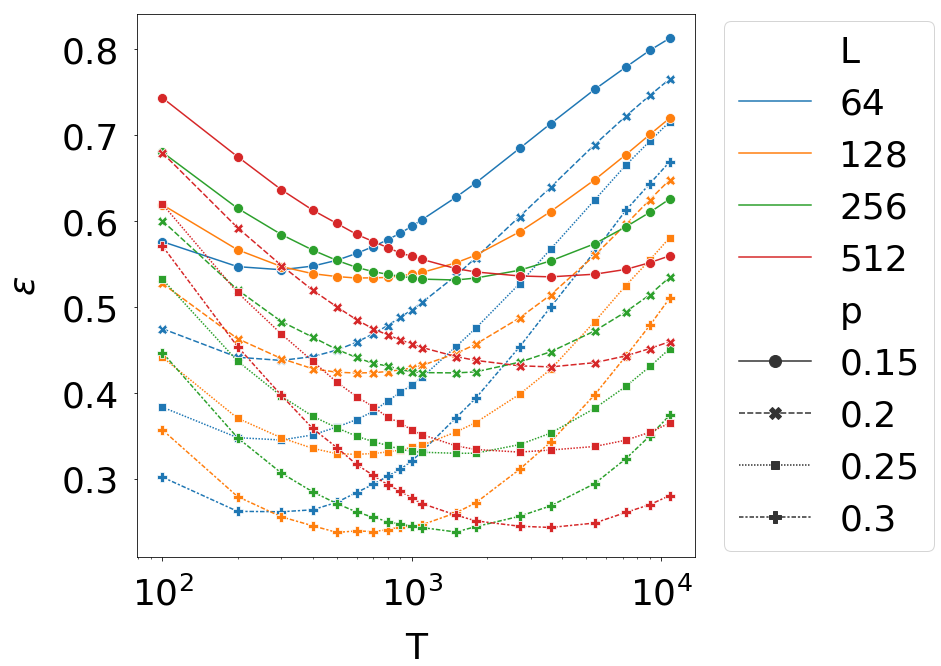
\includegraphics[width=\textwidth]{manna_t_267}
		\caption{Модель Манна, $\gamma=2.67$}
		\label{pic:manna_t_267}
	\end{subfigure}
	\begin{subfigure}[b]{0.45\textwidth}
		\centering
		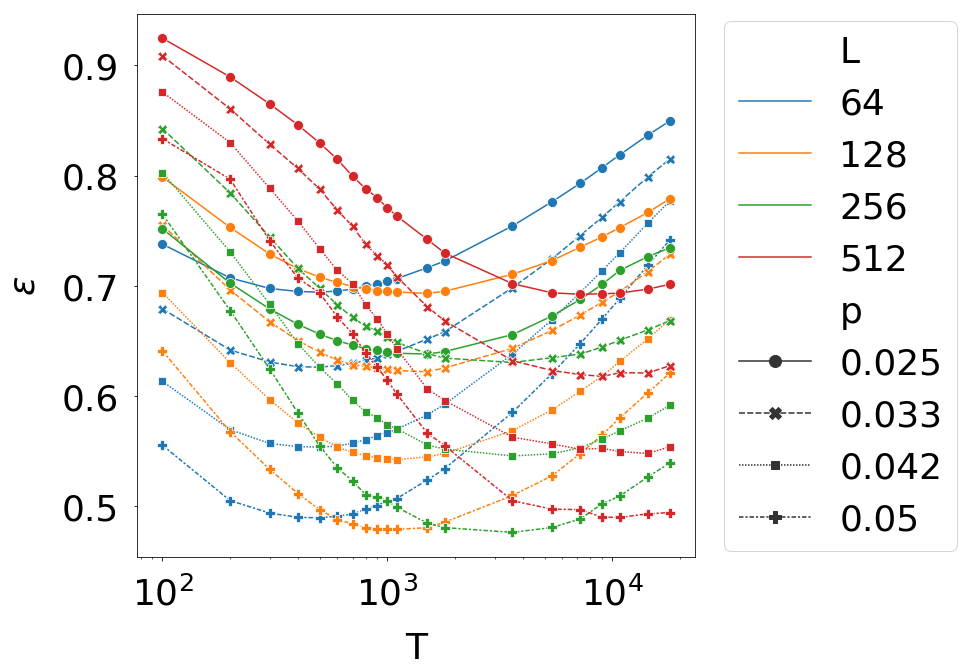
\includegraphics[width=\textwidth]{btw_t_293}
		\caption{Модель БТВ, $\gamma=2.93$}
		\label{pic:btw_t_293}
	\end{subfigure}
	\caption{Качество модели в зависимости от параметра $T$}
	\label{pic:t(L)}
\end{figure}

Формула для переменной принятия решения $y$ похожа на AR(1)-процесс. Поэтому мы ожидаем, что параметр $T$ отвечает за объем памяти в данной модели: чем больше память $T$, тем большее влияние имеет история предыдущих событий, что позволит увеличить качество модели. В то же время, слишком большая память может заставить алгоритм не делать акцент на последних событиях, из-за чего возможны потери в точности.

Численные эксперименты из Приложений \eqref{appendix:a} и \eqref{appendix:b} с разными параметрами $L$, $\gamma$ и $p$ подтвердили наше предположение  о влиянии параметра $T$. Форма кривой $\epsilon_{L, p, \gamma}(T)$ одинаковая для любых $L$, $\gamma$ и $p$ как в модели Манна, так и в модели БТВ, и имеет вид выпуклой функции с единственным пологим минимумом, как на Рис.~\eqref{pic:t(L)}. При том в модели Манна точка минимума не зависит от констант $p$ и $\gamma$, а зависит лишь от размера решетки $L$. Однако, в модели БТВ точка минимума зависит от $\gamma$ и остается независимой от $p$. Эмпирически мы пришли к выводу, что оптимальной $T(L)$ в модели Манна можно считать функцию $T(L) = 300 \cdot 2.25^{\log_{2}\frac{L}{64}}$, в модели БТВ для $\gamma=2.93$ функцию $T(L) = 500 \cdot 2.75^{\log_{2}\frac{L}{64}}$, а для $\gamma=3$ функцию $T(L) = 400 \cdot 2.5^{\log_{2}\frac{L}{64}}$.

\clearpage
\subsection{Скейлинг в модели Манна}

\begin{figure}[h]
	\centering
	\hspace{-25mm}
	\begin{subfigure}[t]{0.27\textwidth}
		\centering
		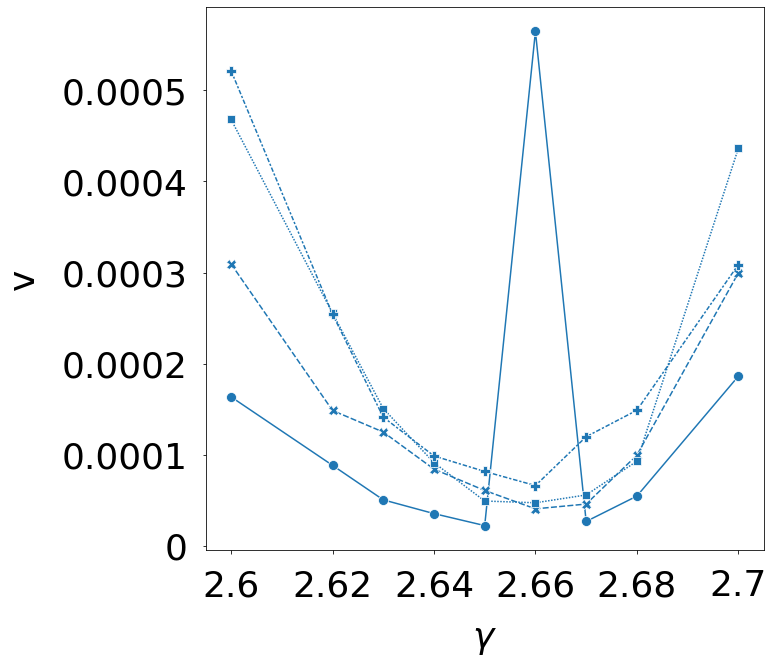
\includegraphics[height=\textwidth]{var_manna}
		\caption{Дисперсия}
	\end{subfigure}
	\hspace{10mm}
	\begin{subfigure}[t]{0.27\textwidth}
		\centering
		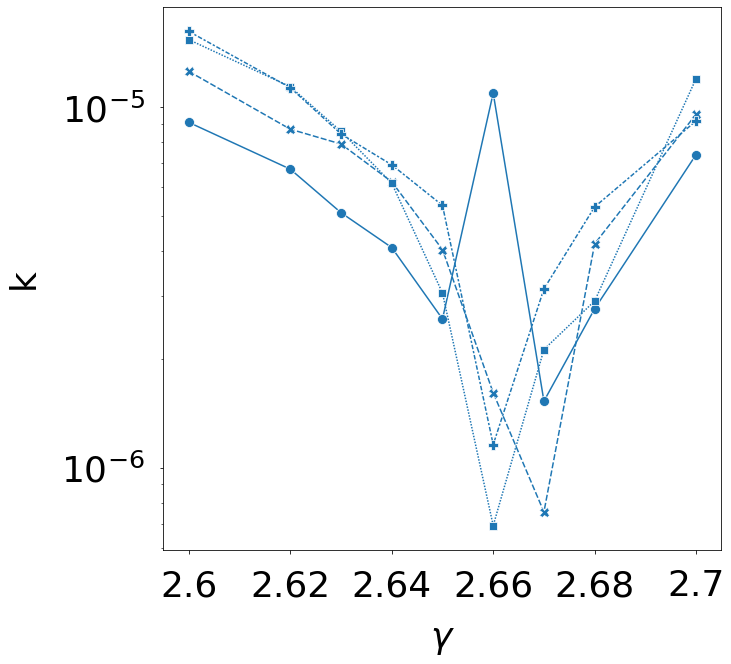
\includegraphics[height=\textwidth]{k_manna}
		\caption{Абсолютное значение коэффициента регрессирующей прямой}
	\end{subfigure}
	\hspace{10mm}
	\begin{subfigure}[t]{0.27\textwidth}
		\centering
		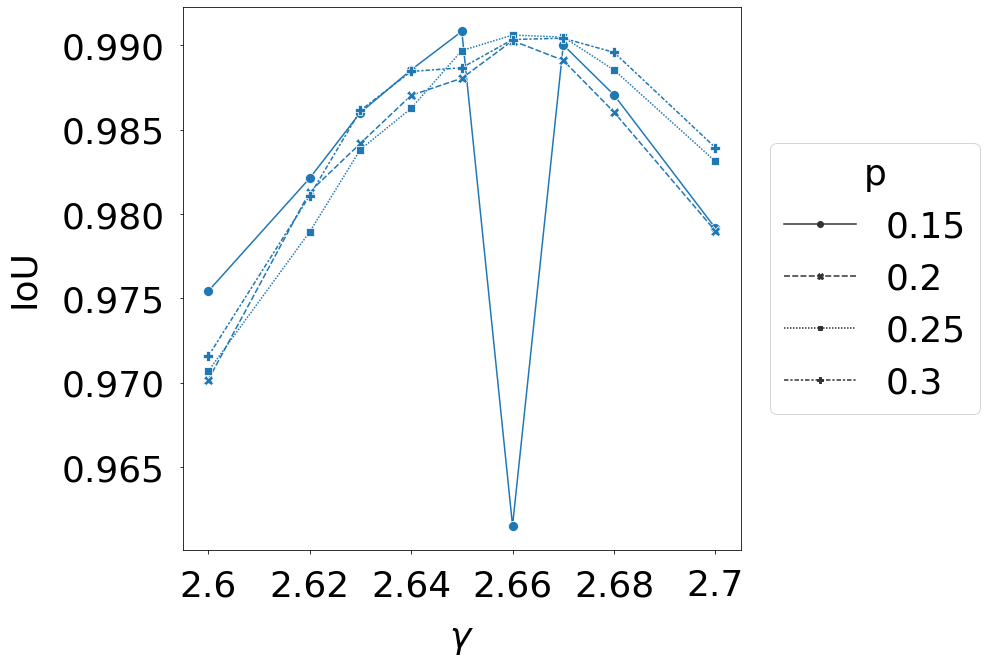
\includegraphics[height=\textwidth]{IoU_manna}
		\caption{IoU}
	\end{subfigure}
	\caption{Метрики качества шкалирования в модели Манна в зависимости от параметра $\gamma$}\label{pic:manna_scaling_metrics}
\end{figure}

Следующей серией численных экспериментов мы установили, что в модели Манна оптимальное $\gamma \approx 2.67$, что подтверждают все три метрики $v(\gamma, p)$, $k(\gamma, p)$ и $IoU(\gamma, p)$ на Рис. \eqref{pic:manna_scaling_metrics}. 

Однако более детальный анализ качества модели с параметром $\gamma = 2.67$ с помощью Рис. \eqref{pic:manna_t_267} показывает, что данный показатель для решетки $L=64$ слишком большой, а для решетки $L=512$ наоборот слишком маленький. Из этого можно сделать вывод, что $\gamma$ должна расти с ростом $L$. Мы считаем, что предельным показателем является $\gamma=2.75$, что согласовывается с показателем шкалирования плотности распределений событий в модели Манна. Дополнительно, мы хотим обратить внимание, что показатель шкалирования плотности распределений событий для таких малых решеток, как у нас, тоже имеет значение $2.67$, а не предельное $2.75$; это видно в экспериментах, отраженных в Приложении \eqref{appendix:d}.

\subsection{Скейлинг в модели БТВ}

\begin{figure}[h]
	\centering
	\centering
	\hspace{-25mm}
	\begin{subfigure}[t]{0.27\textwidth}
		\centering
		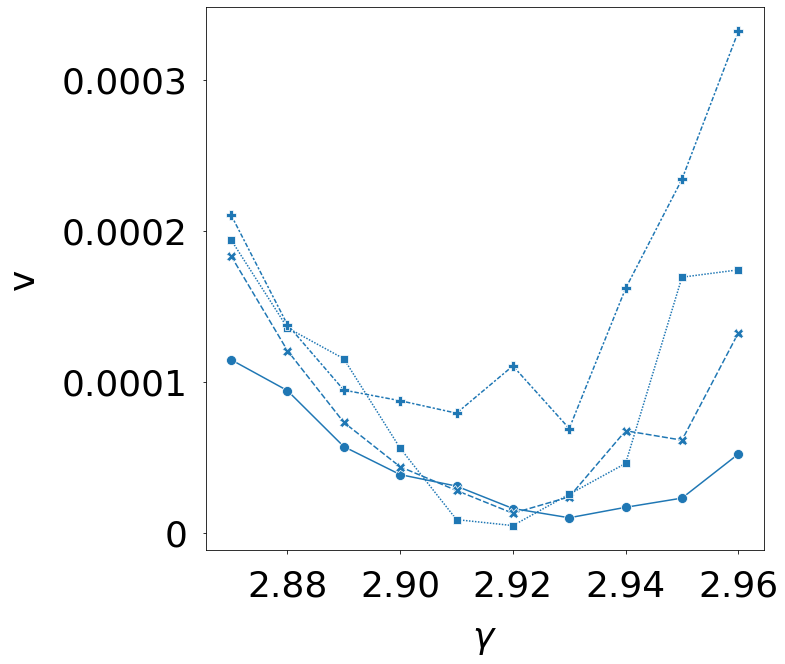
\includegraphics[height=\textwidth]{var_btw}
		\caption{Дисперсия}
	\end{subfigure}
	\hspace{10mm}
	\begin{subfigure}[t]{0.27\textwidth}
		\centering
		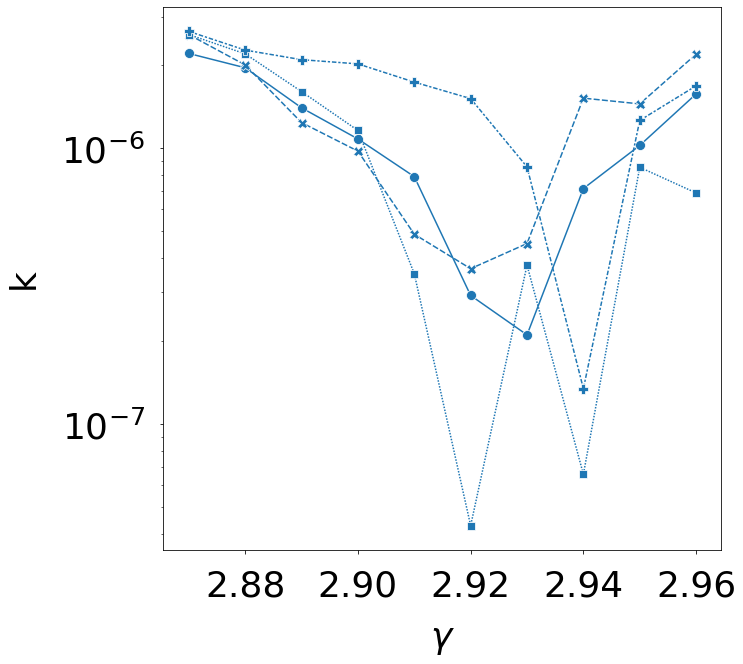
\includegraphics[height=\textwidth]{k_btw}
		\caption{Абсолютное значение коэффициента регрессирующей прямой}
	\end{subfigure}
	\hspace{10mm}
	\begin{subfigure}[t]{0.27\textwidth}
		\centering
		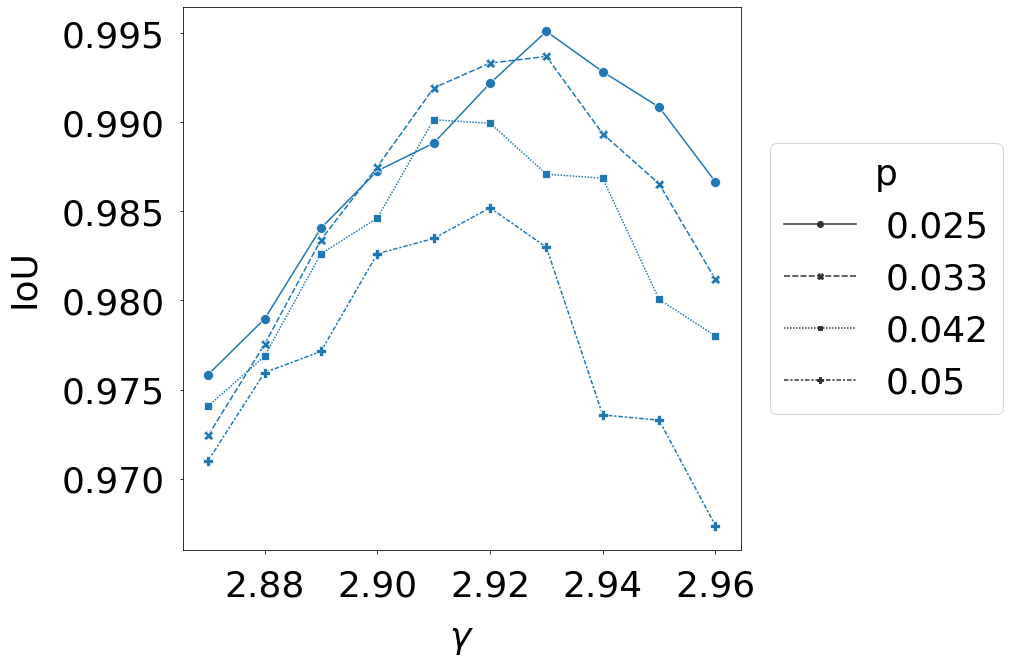
\includegraphics[height=\textwidth]{IoU_btw}
		\caption{IoU}
	\end{subfigure}
	\caption{Метрики качества шкалирования в модели БТВ в зависимости от параметра $\gamma$}\label{pic:btw_scaling_metrics}
\end{figure}

В модели БТВ нам удалось добиться аналогичных результатов: численные эксперименты на Рис. \eqref{pic:btw_scaling_metrics} показывают, что оптимальное $\gamma \approx 2.93$ по всем трем метрикам. Но согласно Рис. \eqref{pic:btw_t_293} мы видим, что для малых решеток показатель должен быть меньше, а для больших --- больше. В работе~\cite{Garber2009} авторы наблюдают такой же показатель для шкалирования размеров максимальных событий $s_{\max}$, и объясняют его эффектом конечного размера. Поскольку теоретическое значение максимального размера события пропорционально $L^3$, мы считаем, что предельным показателем шкалирования является $\gamma=3$.

\subsection{Качество прогноза}

\begin{figure}[h]
	\centering
	\begin{subfigure}[t]{0.45\textwidth}
		\centering
		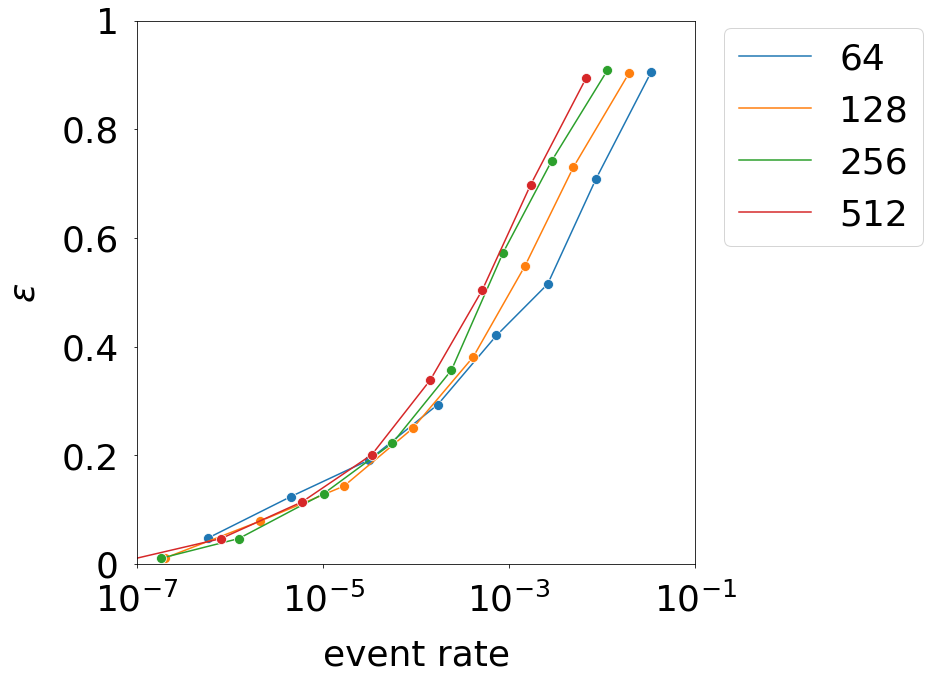
\includegraphics[width=\textwidth]{eps_vs_event_rate_manna}
		\caption{Модель Манна}
		\label{pic:event_rate_manna}
	\end{subfigure}
	\begin{subfigure}[t]{0.45\textwidth}
		\centering
		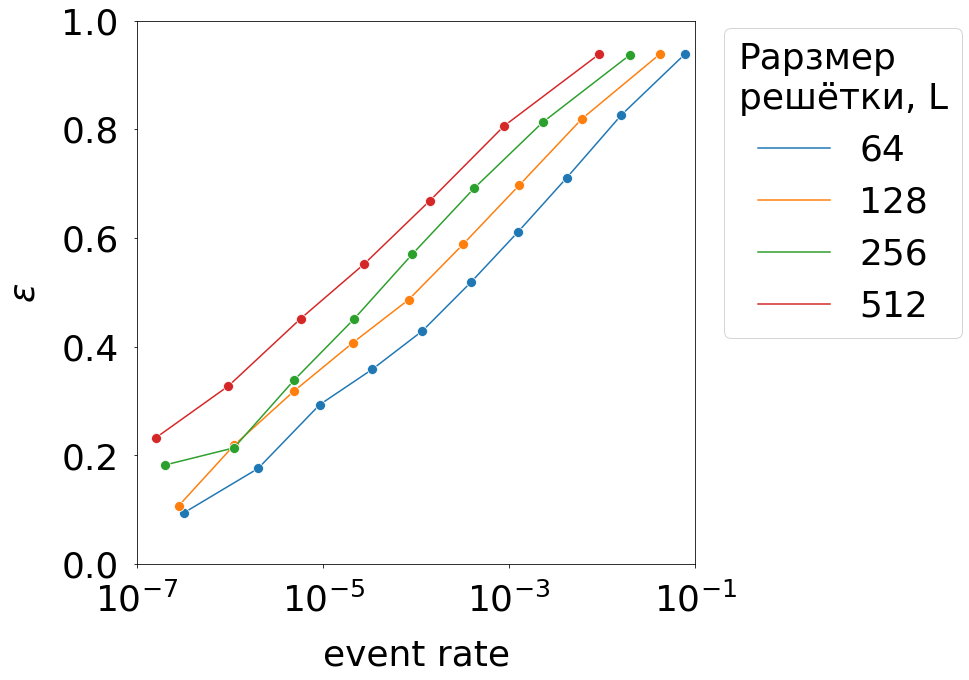
\includegraphics[width=\textwidth]{eps_vs_event_rate_btw}
		\caption{Модель БТВ}
		\label{pic:event_rate_btw}
	\end{subfigure}
	\caption{Качество прогноза в зависимости от частоты встречаемости событий}\label{pic:event_rate}
\end{figure}

Последним экспериментом мы хотели пронаблюдать качество прогноза $\epsilon$ в зависимости от частоты встречаемости событий $event\ rate$. Обратим внимание, что параметр $\gamma$ влияет лишь на качество скейлинга, и не влияет на график $\epsilon$ против $event\ rate$. Поэтому данная кривая является фундаментальным свойством нашего алгоритма прогнозирования критических событий.

\begin{figure}[h]
	\centering
	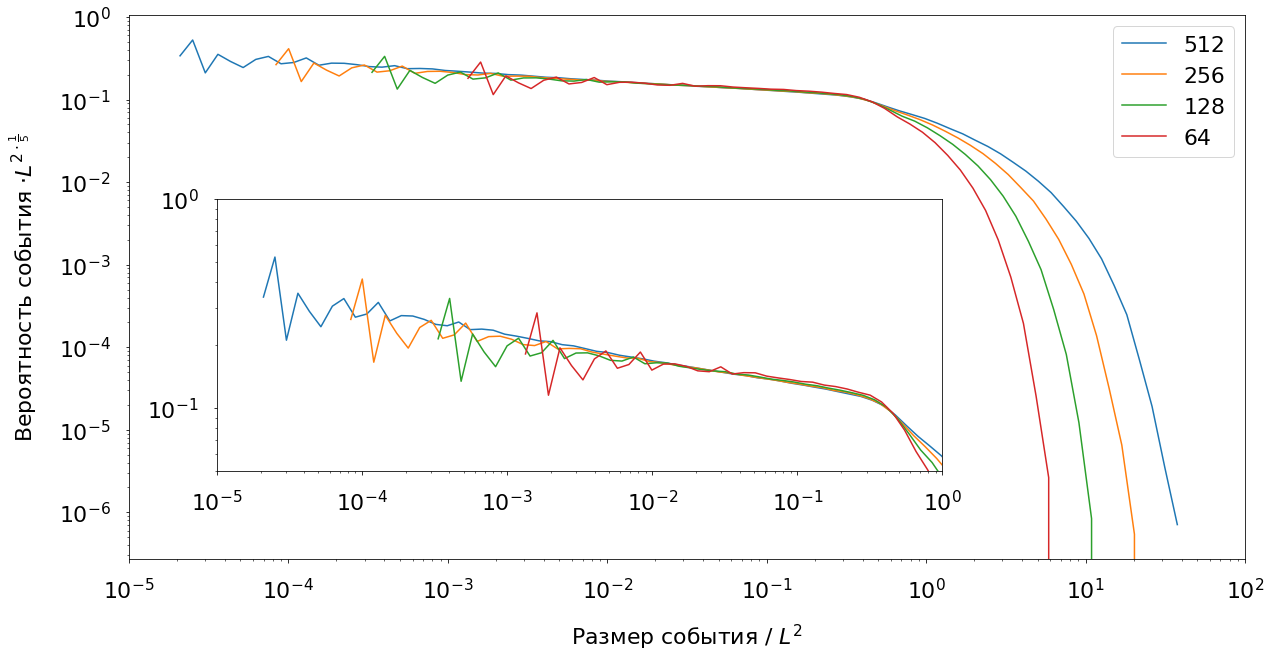
\includegraphics[width=\textwidth]{btw_distribution_200}
	\caption{Шкалирование степенной части в модели БТВ}\label{pic:btw_scaling}
\end{figure}

Результаты в модели Манна показывают, что для достаточно редких событий качество прогноза не зависит от размера решетки $L$. В то же время в модели БТВ качество прогноза падает с ростом $L$ и имеет экспоненциальную зависимость от частоты встречаемости событий. Мы предполагаем, что данный эффект объясняется шкалированием плотностей распределения событий: в модели Манна скейлинг полностью накладывает плотности распределений, как видно в Приложении~\eqref{appendix:d}. В то время как в модели БТВ крупные события, которые мы прогнозируем, шкалируеются как $L^3$, а основная степенная часть --- как $L^2$, что можно наблюдать на Рис.~\eqref{pic:btw_scaling}, и, как следствие, $event\ rate$ падает, если мы хотим сохранять одну и ту же эффективности прогноза с ростом $L$.

	\newpage

    \section{Заключение}
    %Абзац 1 (Мы можем предсказывать в обоих моделях in general). 
В этой работе мы привели пример скейлинг-эффективной модели прогнозирования крупных событий. В отличии от предыдущих результатов, наш алгоритм работает одинаково как для модели Манна, так и для модели БТВ, и имеет тесную связь с известными теоретическими исследованиями. Таким образом, мы собрали все прошлые результаты в стройную схему, которая связывает размеры решетки и эффективность прогнозирования. 

% Абзац 2 (Термодинамические параметры) 
Оказалось, что эффективные параметры для скейлинга событий равны $\gamma=2.75$ в модели Манна и $\gamma=3$ в модели БТВ. Это соответствует показателю шкалирования для плотности распределения событий в модели Манна и показателю шкалирования размера максимального события в модели БТВ соответственно. За счёт этого, в модели Манна для достаточно редких событий качество прогноза не зависит от размера решетки $L$. Однако, в модели БТВ степенная часть имеет отличный от $s_{\max}$ скейлинг, равный $L^2$, из-за этого качество прогноза относительно частоты встречаемости событий падает с ростом размера решетки. Как итог, прогнозировать крупные события в модели Манна получается более эффективно, чем в модели БТВ, и эта разница растет с ростом $L$.

%Абзац 3 (про эффект конечного размера и про то что в реальности показатели не равны термодинамическому пределу). 
На практике численные эксперименты показали, что для решеток малого размера эффективными показателями для скейлинга являются чуть меньшие параметры $\gamma \approx 2.67$ в модели Манна и $\gamma \approx 2.93$ в модели БТВ. Это объясняется эффектом конечного размера решетки, наблюдаемом и на графиках плотности распределения размеров событий. Мы предполагаем, что для наиболее эффективного прогноза стоит плавно увеличивать $\gamma$ с ростом $L$, не достигая термодинамического предела.

%Абзац 4 (Про память).
Крупным событиям в модели песчаной кучи предшествует накопление песка, что на физическом языке означает переход системы из критического в надкритическое состояние. Алгоритм прогноза в данной статье связан с существованием этого перехода. Видимо, на больших временах модель песчаной кучи обладает памятью степенного размера об отсутствии крупных событий. Было бы интересно понять, можно ли существенно поднять качество прогноза за счёт перехода от одной переменной принятия решения $y$, учитывающей память, к вектору переменных принятия решения, сделав модель более сложной, например, с помощью нейронных сетей.


    \newpage

    \phantomsection
    \addcontentsline{toc}{section}{Список литературы}
    \printbibliography
    \newpage

    \appendix
    \section*{Приложения}
\addcontentsline{toc}{section}{Приложения}

\counterwithin{figure}{subsection}
\counterwithin{table}{subsection}
\counterwithin{equation}{subsection}

\renewcommand{\thesubsection}{\Alph{subsection}}

\subsection{Результаты экспериментов в модели Манна}\label{appendix:a}

\begin{figure}[h]
	\centering
	\hspace{-20mm}
	\begin{subfigure}[t]{0.4\textwidth}
		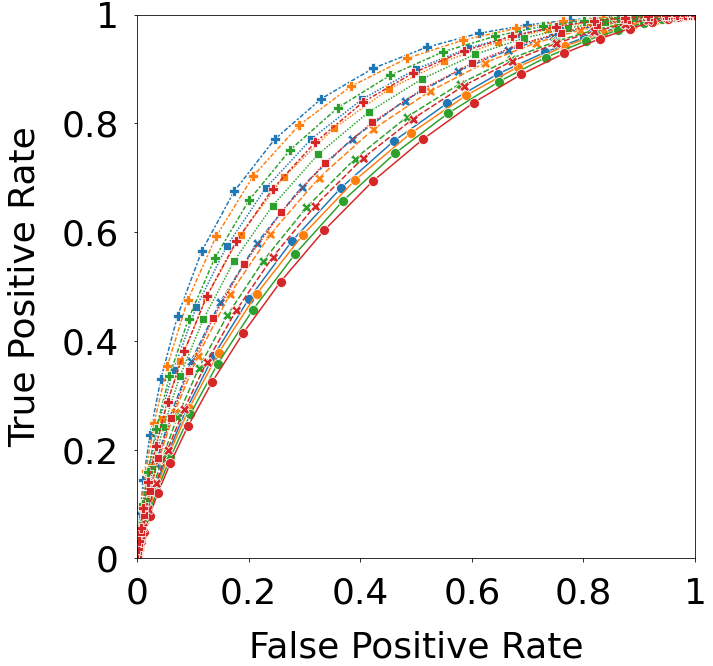
\includegraphics[height=\textwidth]{manna_roc_255} 
		\caption{ROC-кривые}
	\end{subfigure}
	\hspace*{10mm}
	\begin{subfigure}[t]{0.4\textwidth}
		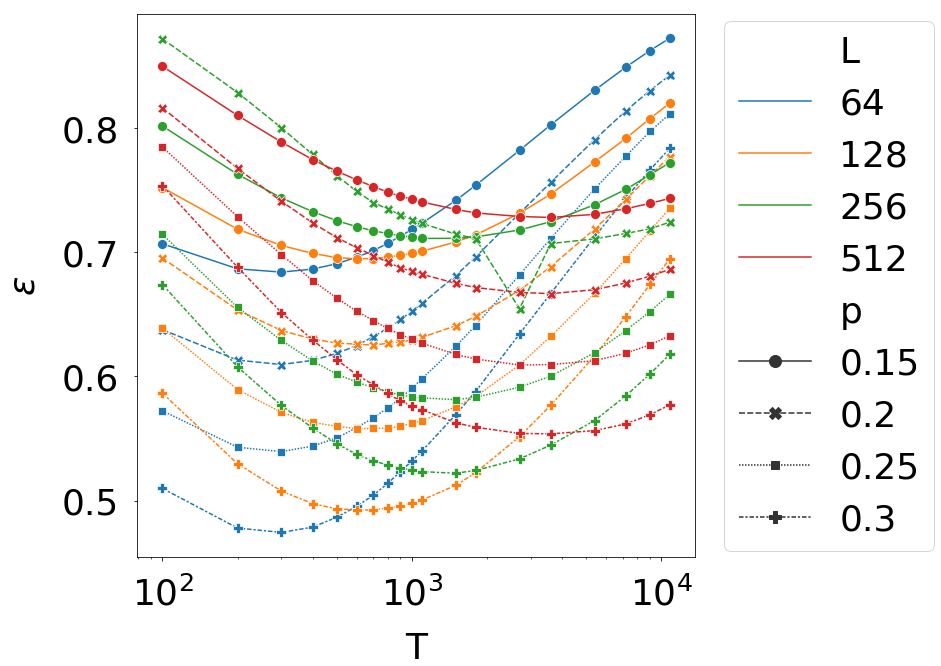
\includegraphics[height=\textwidth]{manna_t_255} 
		\caption{Качество прогноза}
	\end{subfigure}
	\caption{Качество прогноза в зависимости от $T$ для разных констант $p$ и фиксированного параметра $\gamma=2.55$ в модели Манна}
\end{figure}

\begin{figure}[h]
	\centering
	\hspace{-20mm}
	\begin{subfigure}[t]{0.4\textwidth}
		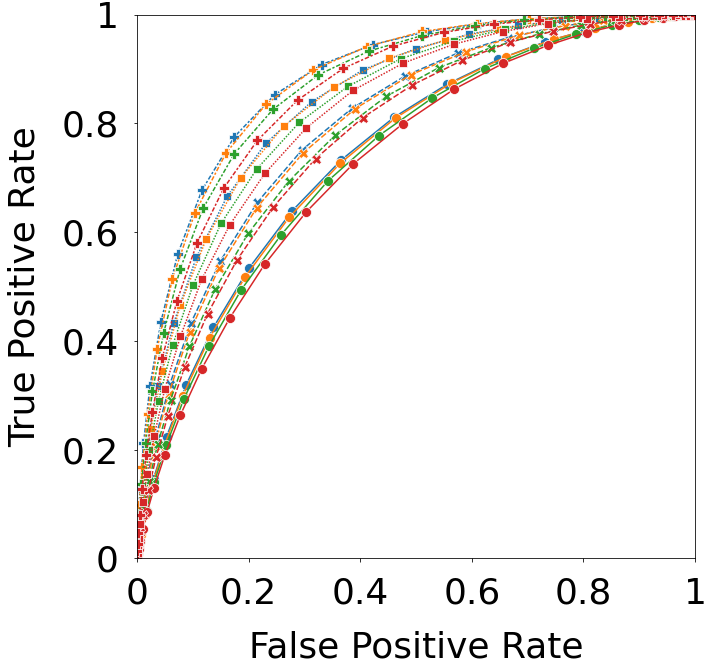
\includegraphics[height=\textwidth]{manna_roc_260} 
		\caption{ROC-кривые}
	\end{subfigure}
	\hspace*{10mm}
	\begin{subfigure}[t]{0.4\textwidth}
		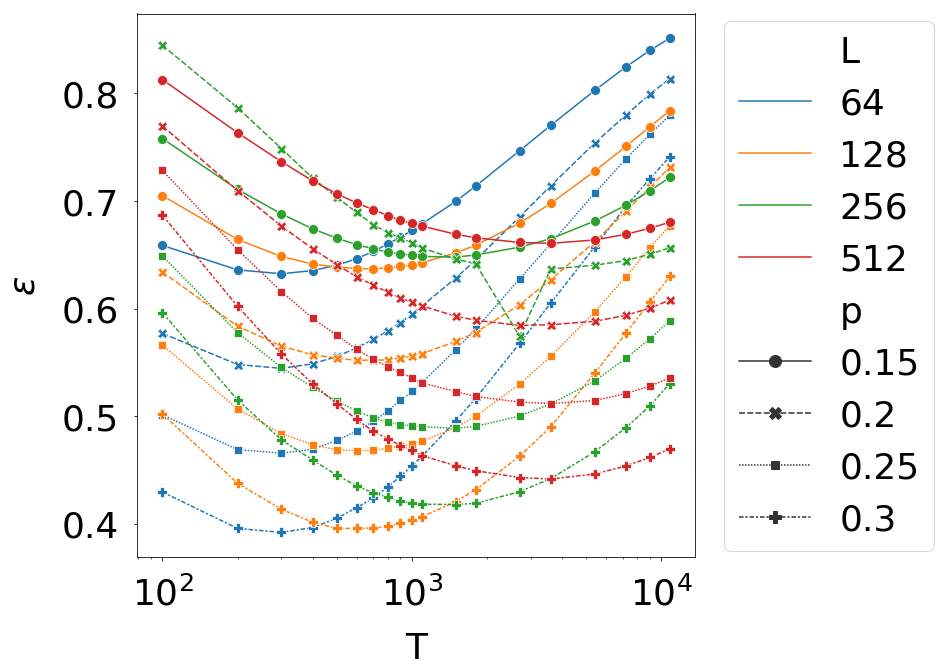
\includegraphics[height=\textwidth]{manna_t_260} 
		\caption{Качество прогноза}
	\end{subfigure}
	\caption{Качество прогноза в зависимости от $T$ для разных констант $p$ и фиксированного параметра $\gamma=2.6$ в модели Манна}
\end{figure}

\begin{figure}[h]
	\centering
	\hspace{-20mm}
	\begin{subfigure}[t]{0.4\textwidth}
		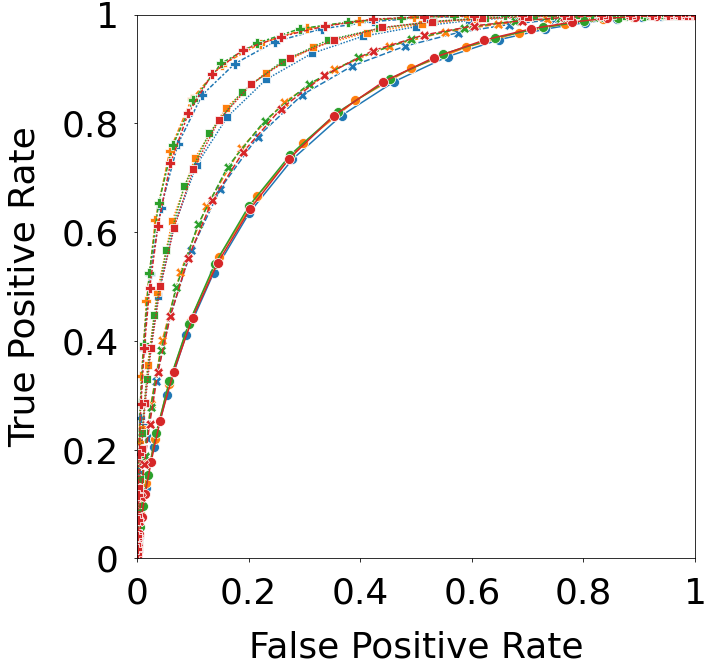
\includegraphics[height=\textwidth]{manna_roc_267} 
		\caption{ROC-кривые}
	\end{subfigure}
	\hspace*{10mm}
	\begin{subfigure}[t]{0.4\textwidth}
		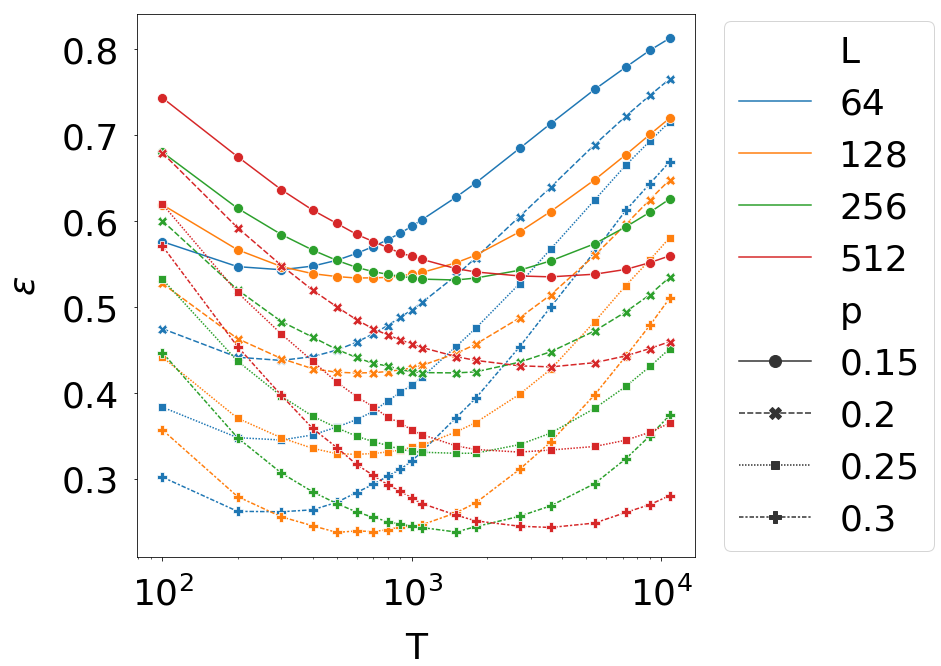
\includegraphics[height=\textwidth]{manna_t_267} 
		\caption{Качество прогноза}
	\end{subfigure}
	\caption{Качество прогноза в зависимости от $T$ для разных констант $p$ и фиксированного параметра $\gamma=2.67$ в модели Манна}
\end{figure}

\begin{figure}[h]
	\centering
	\hspace{-20mm}
	\begin{subfigure}[t]{0.4\textwidth}
		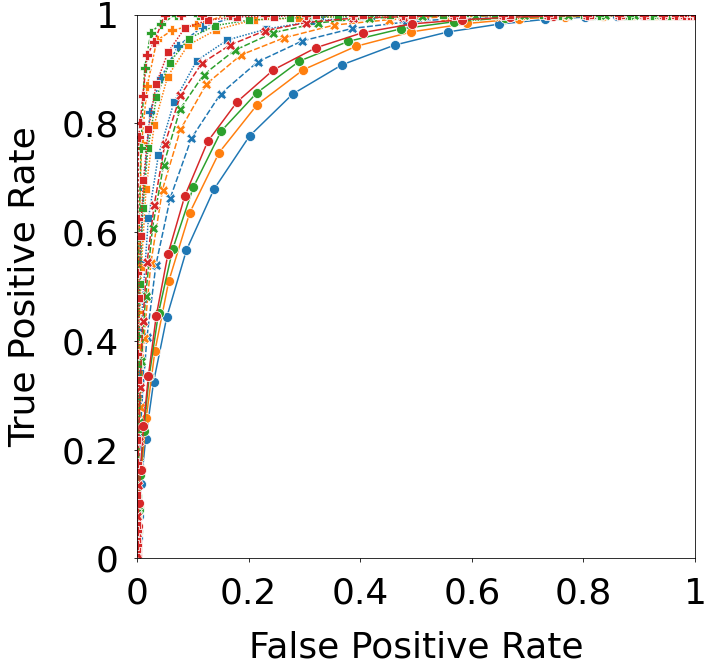
\includegraphics[height=\textwidth]{manna_roc_275} 
		\caption{ROC-кривые}
	\end{subfigure}
	\hspace*{10mm}
	\begin{subfigure}[t]{0.4\textwidth}
		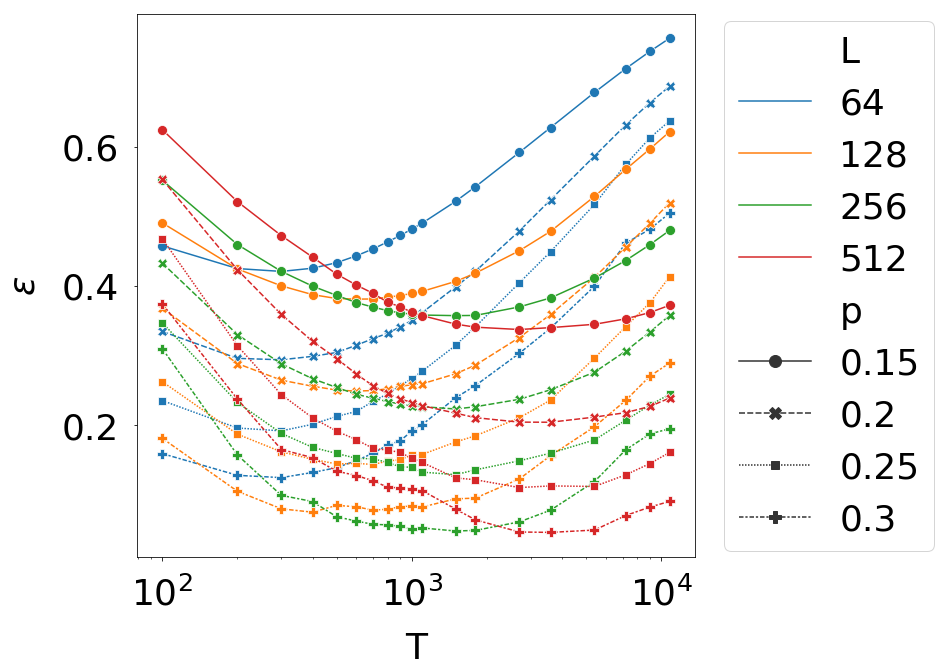
\includegraphics[height=\textwidth]{manna_t_275} 
		\caption{Качество прогноза}
	\end{subfigure}
	\caption{Качество прогноза в зависимости от $T$ для разных констант $p$ и фиксированного параметра $\gamma=2.75$ в модели Манна}
\end{figure}

\newpage
\clearpage

\subsection{Результаты экспериментов в модели БТВ}\label{appendix:b}

\begin{figure}[h]
	\centering
	\hspace{-20mm}
	\begin{subfigure}[t]{0.4\textwidth}
		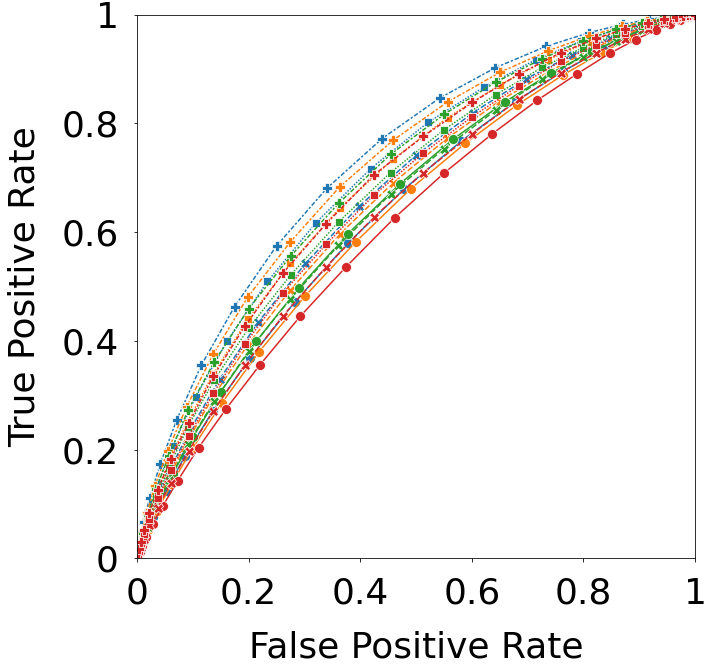
\includegraphics[height=\textwidth]{btw_roc_280} 
		\caption{ROC-кривые}
	\end{subfigure}
	\hspace*{10mm}
	\begin{subfigure}[t]{0.4\textwidth}
		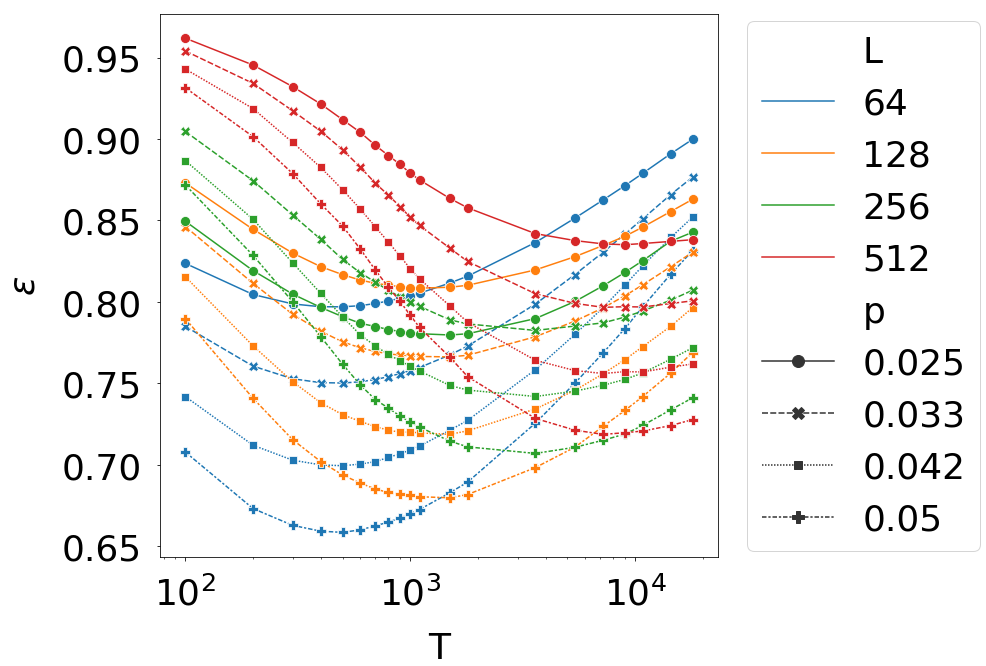
\includegraphics[height=\textwidth]{btw_t_280} 
		\caption{Качество прогноза}
	\end{subfigure}
	\caption{Качество прогноза в зависимости от $T$ для разных констант $p$ и фиксированного параметра $\gamma=2.8$ в модели БТВ}
\end{figure}

\begin{figure}[h]
	\centering
	\hspace{-20mm}
	\begin{subfigure}[t]{0.4\textwidth}
		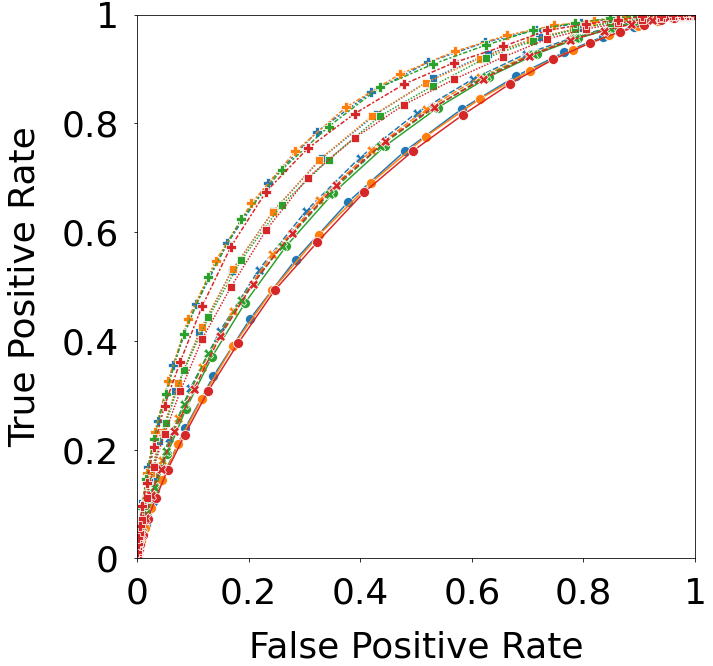
\includegraphics[height=\textwidth]{btw_roc_290} 
		\caption{ROC-кривые}
	\end{subfigure}
	\hspace*{10mm}
	\begin{subfigure}[t]{0.4\textwidth}
		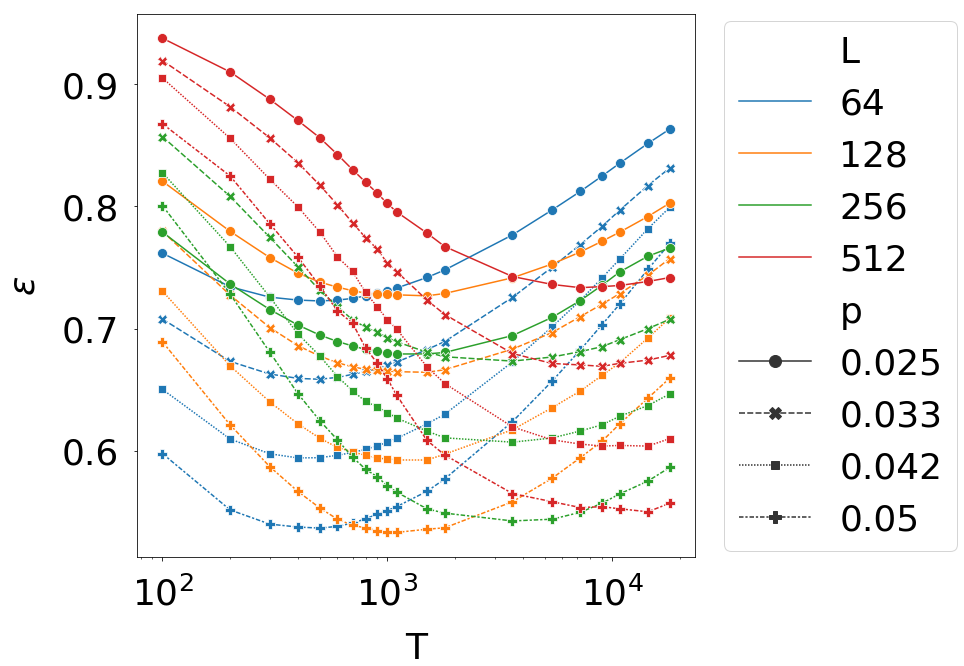
\includegraphics[height=\textwidth]{btw_t_290} 
		\caption{Качество прогноза}
	\end{subfigure}
	\caption{Качество прогноза в зависимости от $T$ для разных констант $p$ и фиксированного параметра $\gamma=2.9$ в модели БТВ}
\end{figure}

\begin{figure}[h]
	\centering
	\hspace{-20mm}
	\begin{subfigure}[t]{0.4\textwidth}
		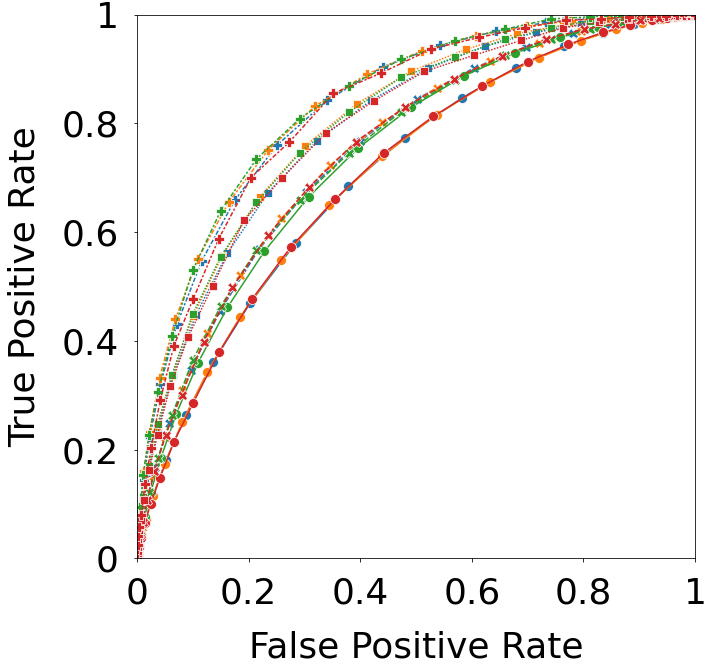
\includegraphics[height=\textwidth]{btw_roc_293} 
		\caption{ROC-кривые}
	\end{subfigure}
	\hspace*{10mm}
	\begin{subfigure}[t]{0.4\textwidth}
		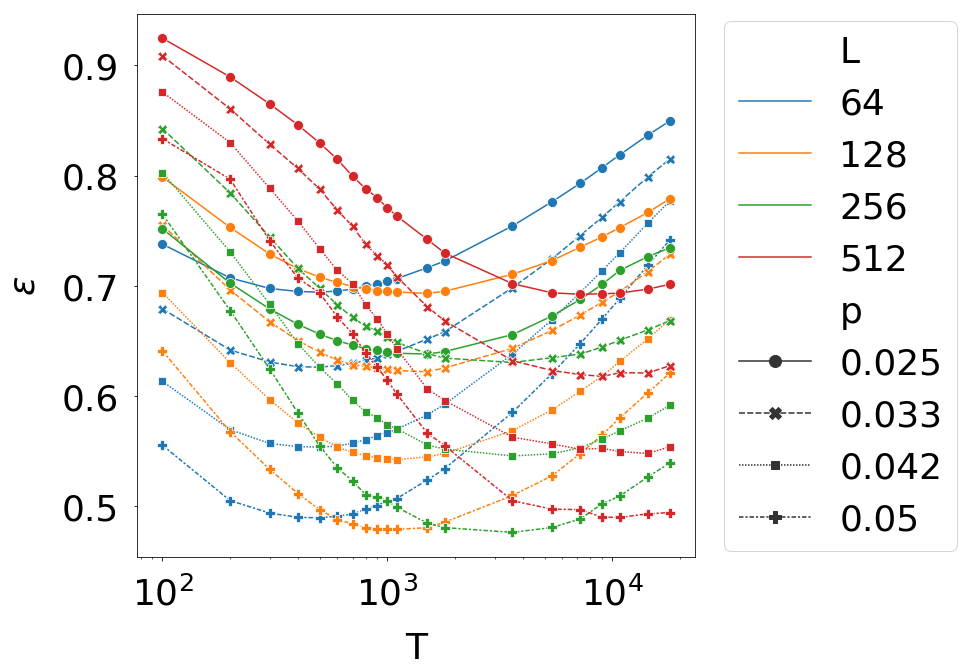
\includegraphics[height=\textwidth]{btw_t_293} 
		\caption{Качество прогноза}
	\end{subfigure}
	\caption{Качество прогноза в зависимости от $T$ для разных констант $p$ и фиксированного параметра $\gamma=2.93$ в модели БТВ}
\end{figure}

\begin{figure}[h]
	\centering
	\hspace{-20mm}
	\begin{subfigure}[t]{0.4\textwidth}
		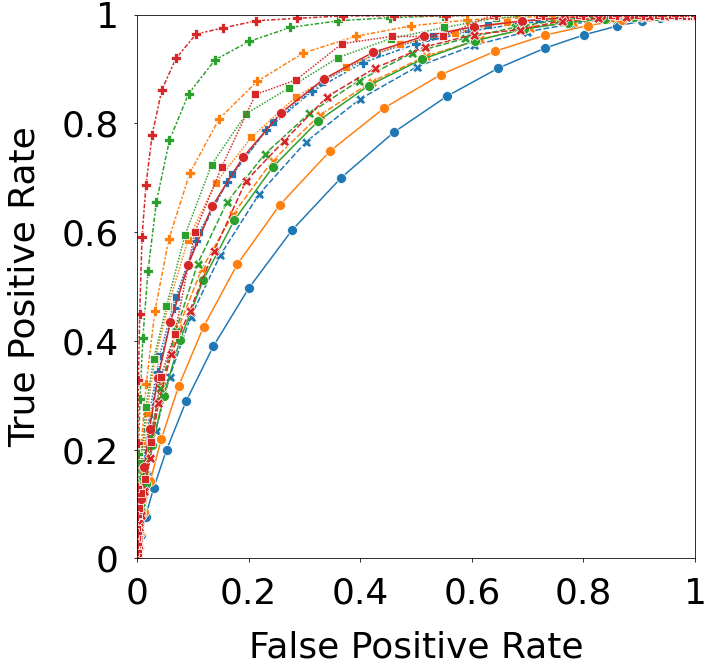
\includegraphics[height=\textwidth]{btw_roc_300} 
		\caption{ROC-кривые}
	\end{subfigure}
	\hspace*{10mm}
	\begin{subfigure}[t]{0.4\textwidth}
		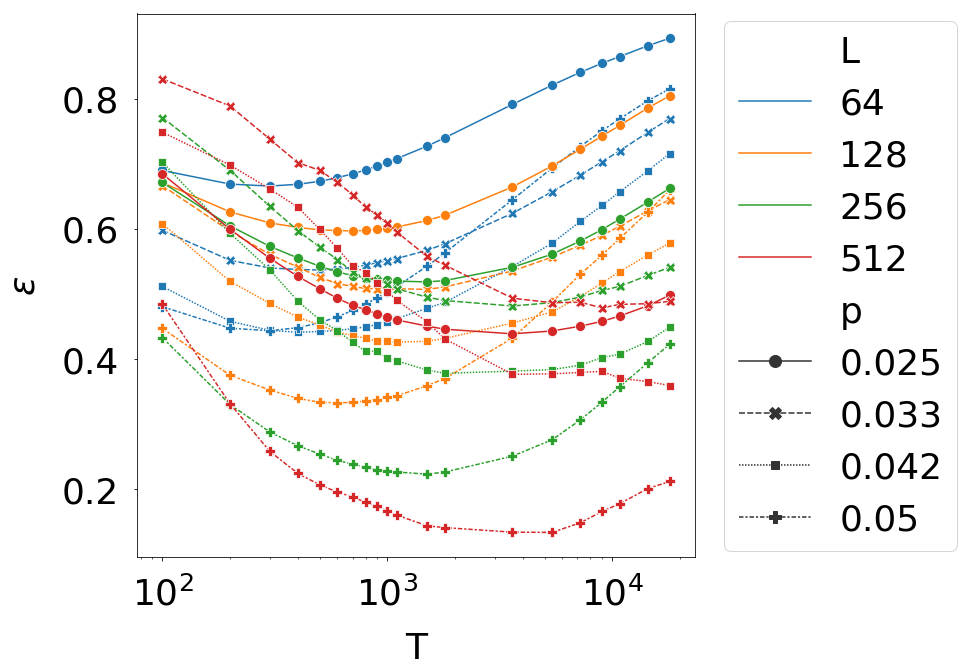
\includegraphics[height=\textwidth]{btw_t_300} 
		\caption{Качество прогноза}
	\end{subfigure}
	\caption{Качество прогноза в зависимости от $T$ для разных констант $p$ и фиксированного параметра $\gamma=3$ в модели БТВ}
\end{figure}

\newpage
\clearpage

\subsection{Количество прогнозируемых событий}\label{appendix:c}
\begin{table}[h]
	\caption{Количество прогнозируемых событий в модели БТВ для заданных констант $p$ и размеров решеток $L$}
	\begin{tabular}{cc}
		$\gamma = 2.93$ & $\gamma = 3$ \\
		\begin{tabular}{l|rrrr}
			\toprule
			p &     64  &    128 &    256 &   512 \\
			\midrule
			0.025 &  173167 &  61170 &  23634 &  9544 \\
			0.033 &   75863 &  24653 &   9117 &  3684 \\
			0.042 &   30507 &   9244 &   3201 &  1265 \\
			0.050 &   13563 &   3779 &   1300 &   528 \\
			\bottomrule
		\end{tabular} &
		\begin{tabular}{l|rrrr}
			\toprule
			p &    64  &    128 &   256 &   512 \\
			\midrule
			0.025 &  72492 &  19542 &  5910 &  1841 \\
			0.033 &  24616 &   5706 &  1531 &   458 \\
			0.042 &   7155 &   1403 &   347 &    75 \\
			0.050 &   2346 &    366 &    82 &    10 \\
			\bottomrule
		\end{tabular}
	\end{tabular}
\end{table}

\begin{table}[h]
	\caption{Количество прогнозируемых событий в модели Манна для заданных констант $p$ и размеров решеток $L$}
	\begin{tabular}{cc}
		$\gamma = 2.67$ & $\gamma = 2.75$ \\
		\begin{tabular}{l|rrrr}
			\toprule
			p &     64  &    128 &    256 &    512 \\
			\midrule
			0.15 &  108114 &  70910 &  47169 &  32008 \\
			0.20 &   43514 &  30106 &  21248 &  15164 \\
			0.25 &   16146 &  11885 &   9042 &   6802 \\
			0.30 &    5253 &   4116 &   3487 &   2879 \\
			\bottomrule
		\end{tabular}
		&
		\begin{tabular}{lrrrr}
			\toprule
			p &    64  &    128 &    256 &   512 \\
			\midrule
			0.15 &  36614 &  20603 &  11990 &  7117 \\
			0.20 &   8569 &   4598 &   2787 &  1674 \\
			0.25 &   1554 &    839 &    507 &   299 \\
			0.30 &    225 &    106 &     62 &    40 \\
			\bottomrule
		\end{tabular}
	\end{tabular}
\end{table}

\newpage
\clearpage

\subsection{Распределение событий в модели Манна}\label{appendix:d}

\begin{figure}[h]
	\centering
	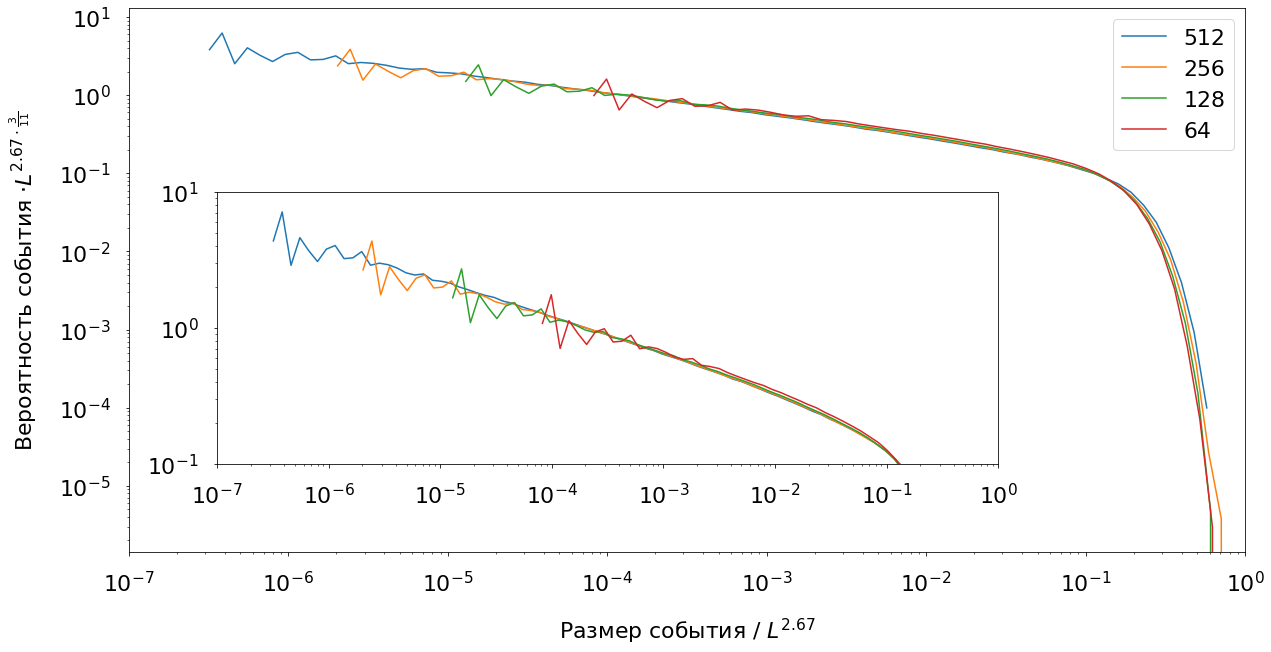
\includegraphics[width=\textwidth]{manna_distribution_267}
	\caption{Распределение событий в модели Манна с нормировкой $\gamma=2.67$}
\end{figure}

\begin{figure}[h]
	\centering
	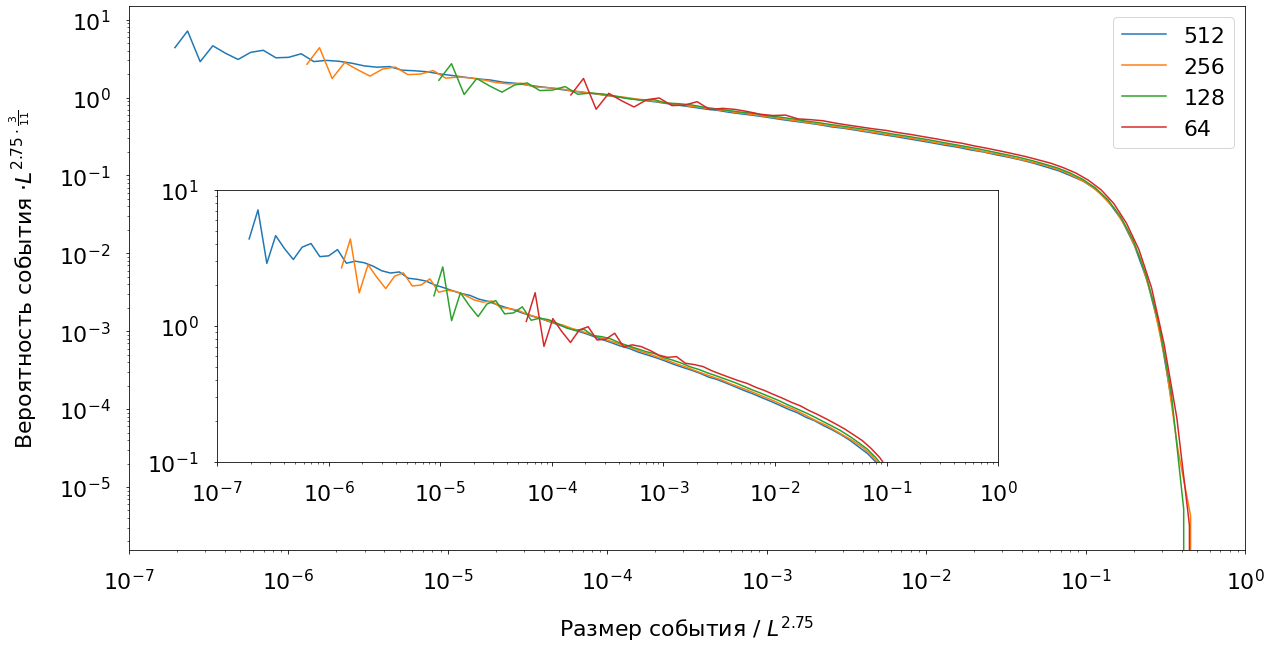
\includegraphics[width=\textwidth]{manna_distribution_275}
	\caption{Распределение событий в модели Манна с нормировкой $\gamma=2.75$}
\end{figure}

\end{document}
